% begin module limit-ex3
\begin{frame}
\begin{example}[Example 3, p. 98]
\begin{columns}[c]
\column{.5\textwidth}
\uncover<6->{
\psset{xunit=1.5cm,yunit=1.5cm}
\begin{pspicture}(-2,-0.5)(2.2,1.5)
\psframe*[linecolor=white](-2, -0.5)(2.2, 1.7)
\psaxes[ticks=none, labels=none]{<->}(0,0)(-2,-0.5)(2,1.5)
\rput[b](0, 1.52){\tiny $y$}
\rput[l](2.02, 0){\tiny $x$}
\rput[br](-0.1,1.1){ $1$}
\psplot[linecolor=red]{-2}{2}{ x 57.295779513 mul sin x div}
\psHollowDot{0}{1}
\end{pspicture}
%\ 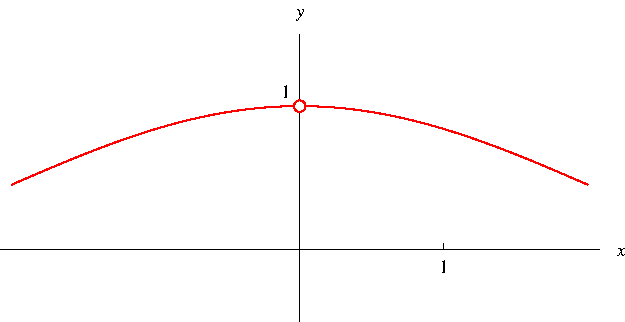
\includegraphics[height=3cm]{limits/pictures/02-01-ex3.pdf}%
}
\column{.5\textwidth}
\begin{itemize}
\item  Guess the value of $\lim_{x\rightarrow 0}\frac{\sin x}{x}$.
\item<2->  Notice that $\frac{\sin x}{x}$ doesn't exist at $0$.  
\item<3->  It does exist at values near $0$.
\item<5->  We guess that the limit is $1$. 
\item<6->  In this case, our guess is correct.
\end{itemize}
\end{columns}
\uncover<4->{
\[
\begin{array}{|r@{.}l|r@{.}l||r@{.}l|r@{.}l|}
\hline
\multicolumn{2}{|c|}{x} &
\multicolumn{2}{|c||}{f(x)} &
\multicolumn{2}{|c|}{x} &
\multicolumn{2}{|c|}{f(x)} \\
\hline
\pm 1 & 
0 & 
0 & 
841471 & 
\pm 0 & 
1 & 
0 & 
998334 \\ 
\pm 0 & 
5 & 
0 & 
958851 & 
\pm 0 & 
05 & 
0 & 
999583 \\ 
\pm 0 & 
4 & 
0 & 
973546 & 
\pm 0 & 
01 & 
0 & 
999983 \\ 
\pm 0 & 
3 & 
0 & 
985067 & 
\pm 0 & 
005 & 
0 & 
999995 \\ 
\pm 0 & 
2 & 
0 & 
993347 & 
\pm 0 & 
001 & 
0 & 
999999 \\ 
\hline
\end{array}
\]
}
\end{example}
\end{frame}
% end module limit-ex3
